\documentclass[11pt,a4paper]{article}

\usepackage[ngerman]{babel}
\usepackage{amsmath}
\usepackage{amssymb}
\usepackage{booktabs}
\usepackage[a4paper,margin=2.5cm]{geometry}
\usepackage{microtype}
\usepackage[htt]{hyphenat}
\usepackage{graphicx}
\usepackage{float}
\usepackage{caption}
\usepackage{xcolor}
\usepackage[hidelinks]{hyperref}

\graphicspath{{figs/}}
\captionsetup{font=small,labelfont=bf}

\definecolor{linkblue}{HTML}{0B4A8A}

\title{\bfseries A2C auf Transportaktien --- Update-Report\\[0.4em]
       \large Stand 7.\ Oktober 2026}
\author{Christopher Voizard}
\date{7.\ Oktober 2026}

\begin{document}

\maketitle
\thispagestyle{empty}

\vfill
\begin{quote}
\textbf{Einordnung vorab:} Alle Ergebnisse dieses Reports stammen aus einem \emph{Nachbau}
in einer anderen Umgebung als das Original-Notebook. Die Abweichungen sind in
Abschnitt~\ref{sec:abweichungen} vollständig dokumentiert und betreffen unter anderem die
Zahl der Input-Features (334 statt 205) sowie die Bibliotheksversionen. Die Zahlen sind
deshalb \emph{nicht} 1:1 mit dem Notebook vergleichbar, sondern als unabhängige
Plausibilitätsprüfung zu lesen.
\end{quote}
\vfill

\newpage
\tableofcontents
\newpage

\section{Kennzahlen-Update (Fundamentaldaten)}

Methodik wie im Notebook: P/E = trailing PE, P/S = trailing PS, Log-Return = Summe der
Tages-Log-Returns des adjustierten Schlusskurses über zwölf Monate.

\begin{table}[H]
  \centering
  \caption{Fundamentalkennzahlen: Original-Notebook (2022) gegenüber 7.\ Oktober 2026.}
  \label{tab:kennzahlen}
  \begin{tabular}{lrrr}
    \toprule
    Kennzahl & Boeing (BA) & Airbus (AIR.PA) & Toyota (TM)\\
    \midrule
    P/E 2022        & n/a (KeyError) & 19,887 & 10,375\\
    P/E 2026        & 70,79          & 25,04  & 7,91\\
    P/S 2022        & 1,502          & 1,458  & 0,0063\\
    P/S 2026        & 1,60           & 1,93   & 0,68\\
    Log-Return 2022 & $-0{,}3025$    & $-0{,}1451$ & $-0{,}1486$\\
    Log-Return 2026 & $-0{,}1558$    & $-0{,}0945$ & $-0{,}0743$\\
    \bottomrule
  \end{tabular}
\end{table}

\paragraph{P/E-Verhältnis.} Die Aussage aus dem Notebook wird bestätigt und teils verschärft.
Airbus bleibt über der Richtgröße von 15 ($19{,}9 \rightarrow 25{,}0$), Toyota klar darunter
($10{,}4 \rightarrow 7{,}9$). Boeing liefert erstmals einen Wert: \textbf{70,79} -- eine
extrem hohe Bewertungskennzahl. Das ist eine Aussage über die Bewertung, nicht über den
Kurs.

\paragraph{P/S-Verhältnis.} Das Update hat einen \textbf{Datenfehler im Original-Notebook}
aufgedeckt. Der dort für Toyota berichtete Wert von $0{,}0063$ (im Text als \glqq nahe
null\grqq{} und damit als sehr günstig gewertet) war ein \texttt{yfinance}-Ausreißer. Der
tatsächliche Wert liegt bei \textbf{0,68}: Toyota bleibt der günstigste der drei, aber die
Aussage \glqq nahe null\grqq{} ist falsch. Boeing steht bei 1,60, Airbus bei 1,93.

\paragraph{Log-Returns.} Die Kernaussage hält: Auch im letzten Jahr sind alle drei Aktien
negativ (BA $-15{,}6\,\%$, AIR $-9{,}5\,\%$, TM $-7{,}4\,\%$), Buy-and-Hold hätte also auch
diesmal verloren. Über den längeren Horizont seit dem Ende der Notebook-Daten (August 2022)
stehen jedoch alle drei klar im Plus (BA $+20{,}5\,\%$, TM $+39{,}5\,\%$, AIR $+50$ bis
$+65\,\%$ über fünf Jahre). Das Verlustbild war damit \emph{fensterspezifisch}.

\begin{figure}[H]
  \centering
  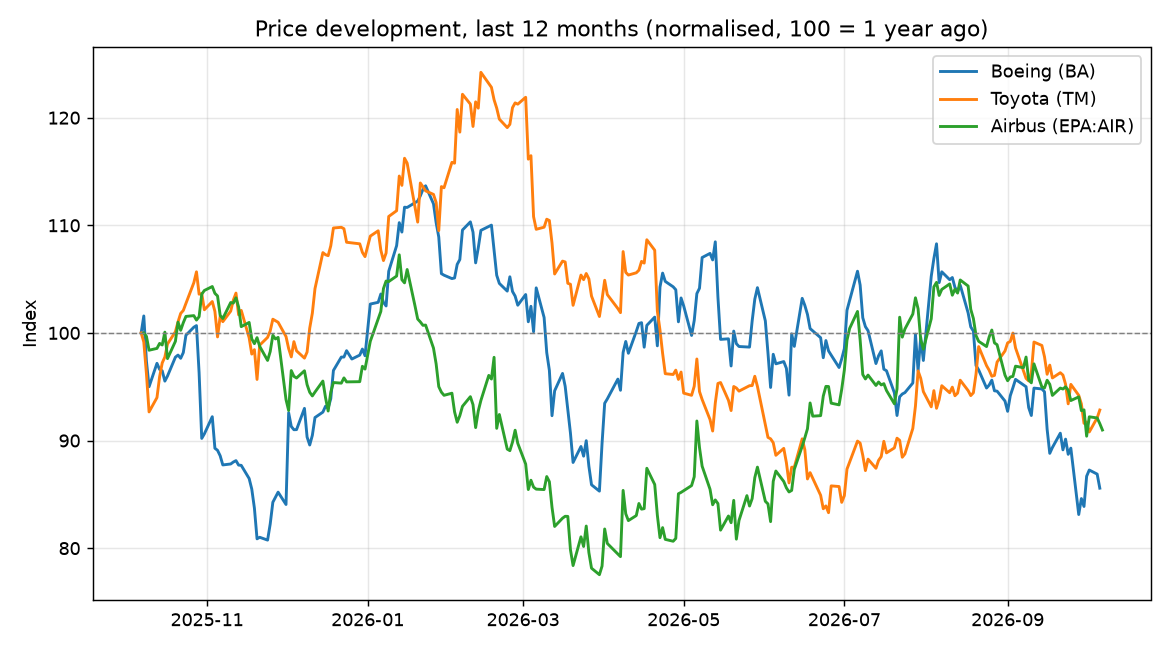
\includegraphics[width=0.80\textwidth]{update_2026_1y.png}
  \caption{Kursentwicklung der drei Aktien über die letzten zwölf Monate
  (normiert, 100 = vor einem Jahr).}
\end{figure}

\section{A2C-Nachbau auf neuen Daten (Boeing)}

\textbf{Protokoll (aus dem Notebook übernommen):} fünf Agenten mit dem Algorithmus
\texttt{A2C} (Policy \texttt{MlpPolicy}), 75.000 Trainingsschritte je Agent, Auswertung mit
\texttt{ai\_trade\_performance} (\texttt{num\_plays=20}). Der Test-Environment übernimmt die
Merkmalsliste (\texttt{use\_variables}) und den Skalierer des Trainings-Environments. Agent und
Buy-and-Hold laufen auf denselben zwanzig Episoden-Seeds, der Vergleich ist also fair.

\begin{table}[H]
  \centering
  \caption{Zeitfenster des Nachbaus.}
  \label{tab:fenster}
  \begin{tabular}{lll}
    \toprule
     & Zeitraum & Datenpunkte\\
    \midrule
    Trainingsfenster (in-sample)   & 06.10.2021 -- 31.05.2024 & ca.\ 660 Handelstage\\
    Testfenster (out-of-sample)    & 01.06.2024 -- 06.10.2026 & ca.\ 580 Handelstage\\
    \bottomrule
  \end{tabular}
\end{table}

\subsection{Ergebnisse je Agent}

End-NAV je Episode (Start $=1{,}0$), Mittel über zwanzig Episoden pro Agent.

\begin{table}[H]
  \centering
  \caption{2026-Nachbau auf Boeing: End-NAV, Mittel über zwanzig Episoden.}
  \label{tab:a2c}
  \begin{tabular}{crrr|rrr}
    \toprule
    \# & Seed & Training Agent & Training B\&H & Test Agent & Test B\&H & Agent besser\\
    \midrule
    1 & 100 & 1,6705 & 0,9647 & \textbf{0,5616} & 0,9475 & 0\,\%\\
    2 & 101 & 2,4073 & 0,9671 & 1,2403 & 0,9408 & 100\,\%\\
    3 & 102 & 4,0534 & 0,9956 & 0,9828 & 0,9412 & 75\,\%\\
    4 & 103 & 7,0580 & 0,9711 & 1,0106 & 0,9493 & 70\,\%\\
    5 & 104 & 5,1547 & 0,9727 & 1,1326 & 0,9485 & 80\,\%\\
    \midrule
    $\varnothing$ & & 4,0688 & 0,9742 & 0,9856 & 0,9455 & 65\,\%\\
    \bottomrule
  \end{tabular}
\end{table}

\subsection{Handelsverhalten}

\begin{table}[H]
  \centering
  \caption{Aktionsverteilung der Agenten (je eine Episode).}
  \label{tab:aktionen}
  \begin{tabular}{crrr|rrr}
    \toprule
    \# & Training short & Training cash & Training long & Test short & Test cash & Test long\\
    \midrule
    1 & 268 & 18  & 348 & 239 & 17  & 299\\
    2 & 295 & 39  & 300 & 304 & 24  & 227\\
    3 & 297 & 24  & 313 & 279 & 29  & 247\\
    4 & 246 & 212 & 176 & 260 & 201 & 94\\
    5 & 296 & 15  & 323 & 309 & 12  & 234\\
    \bottomrule
  \end{tabular}
\end{table}

Alle Agenten handeln überwiegend long; nur Agent~4 hält eine große Cash-Position. Short-Positionen
werden fast immer gehalten, aber selten stark gewichtet.

\subsection{Interpretation}

\paragraph{In-sample ist kein Beleg für Können.} Im Trainingsfenster erreichen die Agenten im
Mittel einen NAV von 4,07 gegenüber 0,97 für Buy-and-Hold und schlagen die Benchmark in
\emph{jeder} Episode. Das ist kein Ergebnis: Hier wurde trainiert und hier wurde gemessen, die
Zahl zeigt nur, dass die Agenten das Fenster auswendig gelernt haben.

\paragraph{Out-of-sample ist das Bild nüchtern.} Im Testfenster liegt der Mittelwert bei
0,9856 gegenüber 0,9455 für Buy-and-Hold, der Agent ist in \textbf{65\,\%} der Episoden
besser -- aber mit sehr großer Streuung: Agent~1 verliert deutlich (0,56), Agent~2 gewinnt
klar (1,24), und zwei von fünf Agenten verlieren in mindestens einem Viertel der Episoden
gegen Buy-and-Hold. Der Vorteil liegt innerhalb der Seed-Streuung und ist
\textbf{nicht signifikant}.

\paragraph{Buy-and-Hold liegt in beiden Fenstern unter 1,0}, Boeing hat also in beiden
Zeiträumen an Wert verloren. Die Frage lautet hier \glqq weniger verlieren\grqq{} statt
\glqq gewinnen\grqq. Insgesamt \textbf{stützt} der Nachbau die Konklusion des Original-Notebooks:
A2C liefert keine verlässliche Outperformance.

\begin{figure}[H]
  \centering
  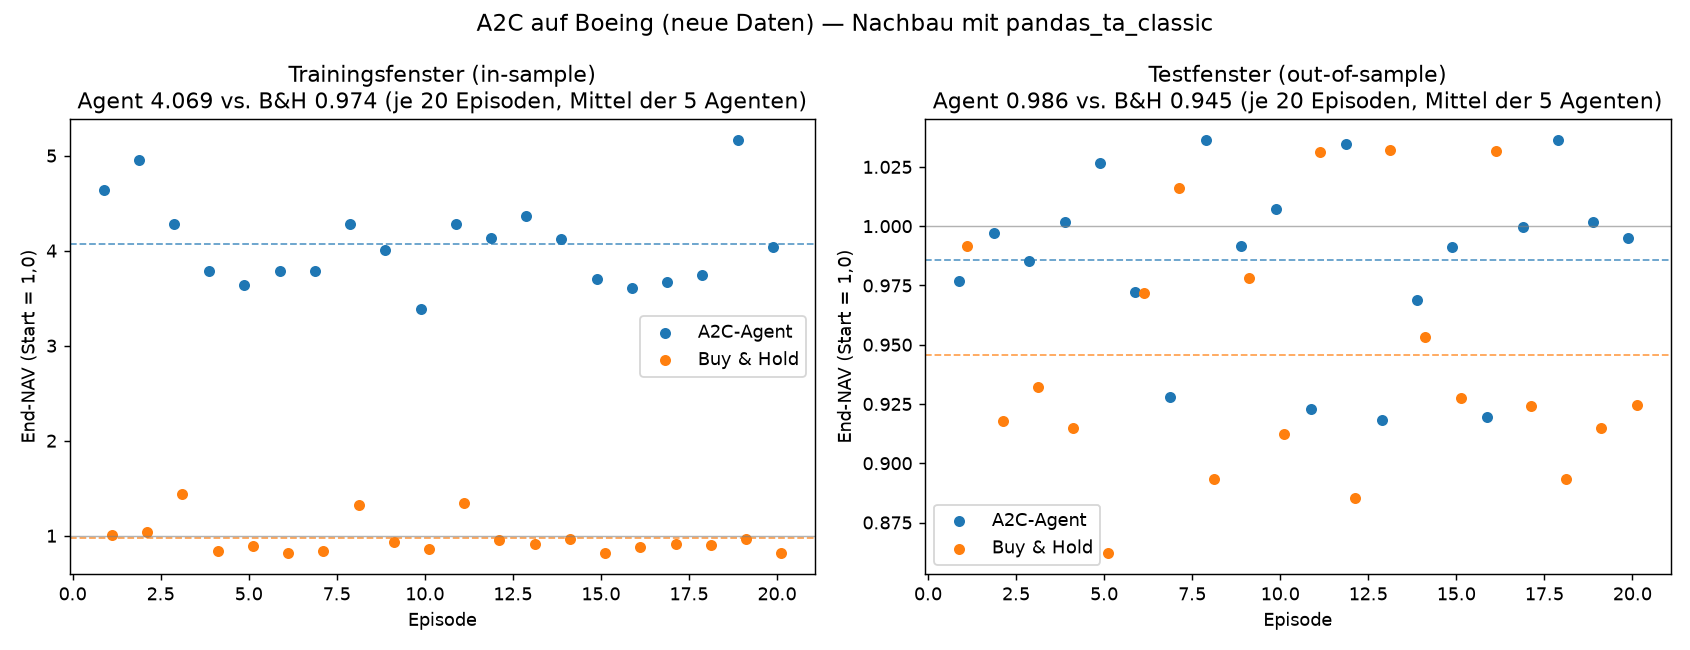
\includegraphics[width=0.98\textwidth]{update_2026_a2c.png}
  \caption{End-NAV je Episode (Mittel der fünf Agenten), links Trainingsfenster
  (in-sample), rechts Testfenster (out-of-sample).}
\end{figure}

\section{Seed-Erweiterung: alle drei Aktien mit 20 Seeds}

\paragraph{Warum überhaupt mehr Seeds?} Abschnitt~\ref{sec:a2c} kommt auf fünf Agenten
(Seeds 100--104). Damit lag der Testvorteil auf Boeing bei $+0{,}04$ NAV-Punkten --- kleiner
als die Streuung zwischen den Agenten. Aus einer so kleinen Stichprobe lässt sich nicht
entscheiden, ob das ein Vorteil oder Rauschen ist. Deshalb wurde das Protokoll unverändert auf
\textbf{20 Seeds (100--119)} erweitert und gleichzeitig auf \textbf{alle drei Aktien} angewandt,
einschließlich Airbus auf den neuen Daten. Die fünf Agenten aus Abschnitt~\ref{sec:a2c} sind
eine Teilmenge dieser zwanzig.

Trainings- und Testfenster sind für alle drei Aktien identisch mit Abschnitt~\ref{sec:a2c}
(06.10.2021--31.05.2024 bzw.\ 01.06.2024--06.10.2026). Verglichen wird jeweils gegen
Buy-and-Hold auf \emph{denselben} zwanzig Episoden-Seeds. Die \emph{Marge} ist die mittlere
gepaarte Differenz Agent $-$ Buy-and-Hold über die Seeds; deren Streuung liefert das
95-%-Konfidenzintervall.

\subsection{Ergebnisse}

\begin{table}[H]
  \centering
  \caption{2026-Nachbau, 20 Seeds je Aktie. End-NAV (Start $=1{,}0$), Mittel über die Seeds;
           $p$ aus dem gepaarten $t$-Test über die Seed-Differenzen ($H_0$: Marge $=0$);
           Trefferquote über alle 400 Episoden je Aktie und Fenster.}
  \label{tab:seeds}
  \small
  \begin{tabular}{llrrrrrr}
    \toprule
    Aktie & Fenster & Agent & Streuung & 95-\%-KI & Buy \& Hold & Marge & $p$\\
    \midrule
    Boeing & Training & 3,669 & 1,400 & [3,01; 4,33] & 0,973 & $\mathbf{+2{,}697}$ & $<0{,}0001$\\
    Boeing & Test     & 1,094 & 0,231 & [0,99; 1,20] & 0,943 & $\mathbf{+0{,}151}$ & $0{,}0037$\\
    Airbus & Training & 1,818 & 0,423 & [1,62; 2,02] & 1,292 & $\mathbf{+0{,}526}$ & $<0{,}0001$\\
    Airbus & Test     & 1,096 & 0,156 & [1,02; 1,17] & 1,091 & $\mathbf{+0{,}005}$ & $0{,}887$\\
    Toyota & Training & 2,455 & 0,724 & [2,12; 2,79] & 1,594 & $\mathbf{+0{,}861}$ & $<0{,}0001$\\
    Toyota & Test     & 0,852 & 0,144 & [0,79; 0,92] & 0,983 & $\mathbf{-0{,}130}$ & $0{,}0001$\\
    \bottomrule
  \end{tabular}
\end{table}

\begin{table}[H]
  \centering
  \caption{Trefferquoten (Anteil der Episoden, in denen der Agent Buy-and-Hold schlägt)
           sowie Rendite/Risiko-Verhältnis im Testfenster.}
  \label{tab:treffer}
  \begin{tabular}{lrrr}
    \toprule
    Aktie & Trefferquote Training & Trefferquote Test & Rendite/Risiko Test (Agent vs.\ B\&H)\\
    \midrule
    Boeing & 100,0\,\% & 75,0\,\% & $0{,}299$ vs.\ $-0{,}160$ \quad ($p=0{,}049$)\\
    Airbus & 79,8\,\%  & 47,8\,\% & $0{,}146$ vs.\ $0{,}322$ \quad ($p=0{,}22$)\\
    Toyota & 87,0\,\%  & 13,8\,\% & $-1{,}038$ vs.\ $0{,}404$ \quad ($p<0{,}0001$)\\
    \bottomrule
  \end{tabular}
\end{table}

\begin{figure}[H]
  \centering
  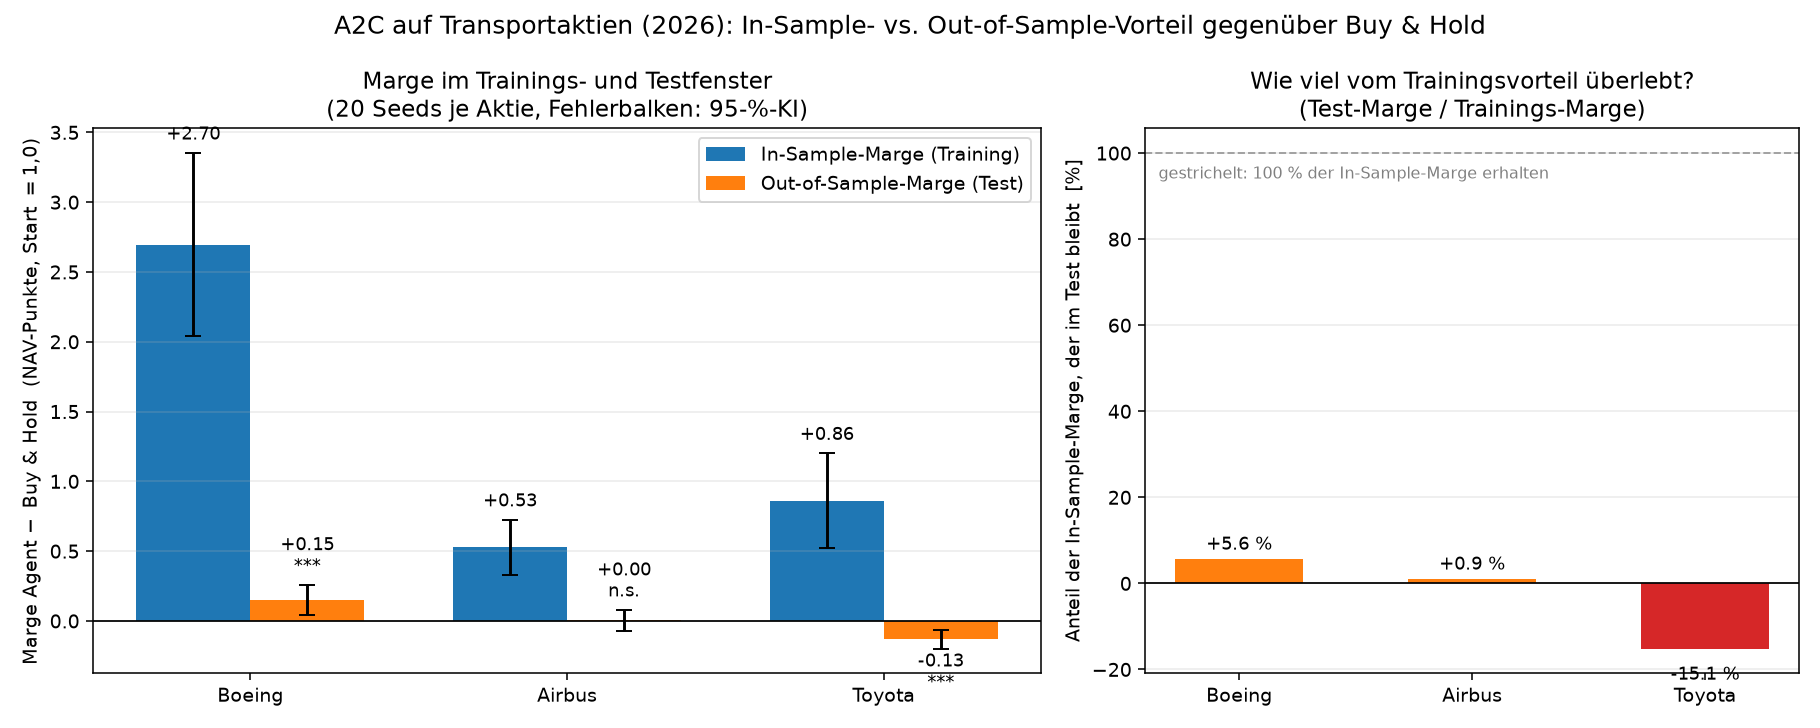
\includegraphics[width=\textwidth]{update_2026_margins.png}
  \caption{Marge (Agent $-$ Buy-and-Hold) im Trainings- und im Testfenster je Aktie.
  Fehlerbalken: 95-\%-Konfidenzintervall der mittleren gepaarten Differenz über 20 Seeds.
  Rechts: Anteil der In-Sample-Marge, der out-of-sample übrig bleibt.}
  \label{fig:margins}
\end{figure}

\subsection{Interpretation}

\paragraph{In-sample schlägt der Agent überall deutlich.} Zwischen $+0{,}53$ und $+2{,}70$
NAV-Punkten, in allen drei Fällen mit $p<0{,}0001$ und Trefferquoten von 80 bis 100\,\%.
Das ist erwartbar und \emph{kein} Beleg für Können: Hier wurde trainiert und hier wurde gemessen.

\paragraph{Out-of-sample bleibt fast nichts übrig.} Boeing behält einen signifikanten Vorteil
($+0{,}151$, $p=0{,}0037$), Airbus landet exakt auf Buy-and-Hold ($+0{,}005$, $p=0{,}89$,
Trefferquote 47,8\,\% --- ein Münzwurf), und Toyota dreht ins Gegenteil
($-0{,}130$, $p=0{,}0001$, Trefferquote 13,8\,\%).

\paragraph{Die In-Sample-Marge sagt den Out-of-Sample-Erfolg nicht vorher.} Toyota war im
Training der zweitbeste und im Test der schlechteste, Airbus im Training der schwächste und im
Test der zweitbeste; die Rangfolge der beiden Fenster hat nichts miteinander zu tun. Anschaulich
rechts in Abbildung~\ref{fig:margins}: von der Trainingsmarge bleiben bei Boeing 5,6\,\%,
bei Airbus 0,9\,\% und bei Toyota $-15{,}1\,\%$.

\paragraph{Die Zahl der Seeds hat ein Urteil gedreht.} Mit fünf Seeds war der Boeing-Testvorteil
($+0{,}040$, Trefferquote 65\,\%) innerhalb der Streuung und damit nicht signifikant; mit zwanzig
Seeds sind es $+0{,}151$ bei $p=0{,}0037$. Dasselbe Experiment, dasselbe Protokoll --- nur eine
belastbare Stichprobe.

\paragraph{Gegenüber dem Original-Notebook (2013--2017)} war dort für alle drei Aktien ein
Agentenvorteil messbar (Toyota 1,27 gegen 1,00 bei 80\,\% Trefferquote). Auf den neuen Daten ist
bei Toyota nichts davon übrig --- es kippt ins signifikant Schlechtere. Das \textbf{stützt} die
Grundaussage des Notebooks, dass A2C keine verlässliche Outperformance liefert, und schärft sie:
Der Nachbau findet keine Aktie, bei der der Vorteil robust groß wäre.

\paragraph{Einschränkungen.} Zwanzig Seeds sind deutlich besser als fünf, aber weiterhin eine
kleine Stichprobe; die Konfidenzintervalle in Tabelle~\ref{tab:seeds} sind entsprechend breit.
Die Airbus-Kursreihe stammt aus einer anderen Quelle als Boeing und Toyota (Yahoo,
\texttt{AIR.PA}, in Euro, 1.307 Handelstage bis 06.10.2026). Und es gilt weiterhin die
Haupteinschränkung aus Abschnitt~\ref{sec:abweichungen}: der Beobachtungsvektor ist mit
\textbf{335} Merkmalen größer als im Original (205), ein Teil der Differenz kann daher stammen.

\section{Methodik-Abweichungen gegenüber dem Original-Notebook}
\label{sec:abweichungen}

Der Nachbau lief \emph{nicht} in der ursprünglichen conda-Umgebung (Python 3.8.8,
stable-baselines3 1.6.0, gym 0.21, torch 1.12.1), sondern in einem Linux-Container mit
aktuellem Stack. Alle Ersetzungen sind bewusst und dokumentiert.

\begin{table}[H]
  \centering
  \caption{Ersetzungen im Nachbau.}
  \label{tab:abweichungen}
  \begin{tabular}{lll}
    \toprule
    Aspekt & Original-Notebook & Nachbau 2026\\
    \midrule
    Kursdaten            & \texttt{yfinance} (live)      & lokale CSV\\
    Technische Indikatoren & \texttt{pandas\_ta} 0.3.14b0 & \texttt{pandas\_ta\_classic}\\
    Zahl der Indikatoren & 204                          & 348\\
    Beobachtungsvektor   & 205                          & \textbf{334}\\
    Parallelisierung     & Multiprocessing-Pool         & seriell\\
    RL-Stack             & SB3 1.6.0 + gym 0.21         & SB3 2.9 + gymnasium 1.4\\
    \bottomrule
  \end{tabular}
\end{table}

\textbf{Die wichtigste Einschränkung ist der Beobachtungsvektor von 334 statt 205.} Der Agent
sieht mehr Input-Features als im Original, ein Teil der Leistungsdifferenz kann also daher
stammen und \emph{nicht} vom Datenupdate. Hinzu kommt: \texttt{yfinance} ist von diesem Host
hart geblockt (HTTP 429 auf allen Endpunkten), weshalb die Kursreihe aus einer lokalen Datei
gelesen wird, und das Helper-Paket \texttt{aif\_course} ist nicht mehr verfügbar
(das Upstream-Repository antwortet mit HTTP 404). Das Environment musste lokal
rekonstruiert werden; die genauen Ersetzungen sind im Begleitcode dokumentiert.

\textbf{Nicht reproduzierbar} ist der Original-Lauf mit den vorab trainierten Agenten
(\texttt{A2C\_showcase\_agent1..5}). Es lag nur \emph{ein} Agent vor, ein Vergleich
\glqq Original-Agent gegen neu trainierter Agent\grqq{} war daher nicht möglich.

\section{A3C: ein zweiter Algorithmus, eine Zerlegung und ein generatives Marktmodell}
\label{sec:a3c}

\paragraph{Woher die Frage kommt.} Original-Notebook und Nachbau (Abschnitt~\ref{sec:a2c})
nutzen \emph{A2C}, also synchrones Lernen. Die naheliegende Gegenprobe ist \emph{A3C}:
mehrere Worker sammeln parallel Rollouts und schieben ihre Gradienten in ein gemeinsames
Netz (Hogwild-Stil, nur der Optimizer-Schritt ist gesperrt). Umgebung, Fenster,
Episoden-Seeds und Auswertungsfunktionen bleiben unverändert --- damit misst der Vergleich
den Lernalgorithmus und nicht das Drumherum. Die Endauswertung läuft wieder über
\textbf{20 Seeds (100--119)}. Eine Besonderheit vorweg: A3C wurde erst
\emph{nach} der Fertigstellung des A2C-Teils gebaut, es gibt also keine
Notebook-Vorlage, gegen die man die Zahlen spiegeln könnte.

\subsection{Die Baseline hat keinen Vorsprung}

\begin{table}[H]
  \centering
  \caption{A3C auf Boeing, 20 Seeds. Marge $=$ Agent $-$ Buy-and-Hold in NAV-Punkten
           (Start $=1{,}0$); $p$ einseitig aus dem $t$-Test ``Marge $>0$''.
           ``R/R'' ist das Rendite/Risiko-Verhältnis im Testfenster.}
  \label{tab:a3c-arms}
  \small
  \begin{tabular}{lrrrrrr}
    \toprule
    Arm & Training & Test & 95-\%-KI Test & Treffer Test & $p$ & R/R Test\\
    \midrule
    Baseline                 & $+8{,}43$ & $+0{,}019$ & $[-0{,}06;+0{,}10]$ & 51,0\,\% & $0{,}32$  & $-0{,}24$\\
    \texttt{ent\_coef} 0,02  & $+8{,}37$ & $+0{,}047$ & $[-0{,}03;+0{,}12]$ & 64,0\,\% & $0{,}10$  & $-0{,}37$\\
    \texttt{obs\_noise} 0,01 & $+8{,}79$ & $+0{,}038$ & $[-0{,}03;+0{,}11]$ & 57,2\,\% & $0{,}14$  & $-0{,}45$\\
    \texttt{nstep} 10        & $+6{,}71$ & $+0{,}125$ & $[+0{,}01;+0{,}24]$ & 67,8\,\% & $0{,}019$ & $-0{,}05$\\
    Bündel (alle drei)       & $+7{,}69$ & $+0{,}145$ & $[+0{,}03;+0{,}26]$ & 70,2\,\% & $0{,}007$ & $-0{,}03$\\
    Bündel $+$ Bootstrap     & $+0{,}02$ & $+0{,}218$ & $[+0{,}09;+0{,}35]$ & 77,8\,\% & $0{,}0012$& $+0{,}50$\\
    \texttt{nstep} 10 $+$ Bootstrap & $+0{,}02$ & $+0{,}218$ & $[+0{,}09;+0{,}35]$ & 72,5\,\% & $0{,}0010$& $+0{,}38$\\
    \bottomrule
  \end{tabular}
\end{table}

Die Baseline wiederholt das A2C-Ergebnis: Im Testfenster liegt die Marge bei
$+0{,}019$ NAV-Punkten, der Agent gewinnt in \textbf{51,0\,\%} der Episoden --- ein
Münzwurf --- und der einseitige $p$-Wert ist $0{,}32$. \textbf{Ein A3C-Agent ohne
Anpassungen hat keinen belegbaren Vorsprung vor Buy-and-Hold.} Im Trainingsfenster steht
gleichzeitig eine Marge von $+8{,}43$: Der Agent hat den einen historischen Pfad
auswendig gelernt.

\subsection{Zerlegung: welcher Faktor trägt?}

Ein naheliegender Griff ins Werkzeugregal ist ein Bündel aus drei Änderungen:
\texttt{nstep} $5\to10$ (n-Schritt-Returns), \texttt{ent\_coef} $0{,}01\to0{,}02$
(Entropie-Bonus) und \texttt{obs\_noise} $0\to0{,}01$ (Gauß-Rauschen auf die Beobachtung
während des Trainings). Das Bündel hebt die Testmarge auf $+0{,}145$
($p=0{,}007$). Nur: \emph{welcher} der drei Faktoren tut das?

Deshalb wurde jeder Faktor einzeln bei ebenfalls 20 Seeds gefahren (Zeilen 2--4 in
Tabelle~\ref{tab:a3c-arms}). Das Ergebnis ist eindeutig und war für mich überraschend:

\paragraph{\texttt{nstep} ist der Wirkstoff.} Allein erreicht \texttt{nstep} $10$
bereits $+0{,}125$ ($p=0{,}019$, Trefferquote 67,8\,\%) --- das sind \textbf{85\,\%} der
Bündelwirkung. Der gepaarte Test Bündel gegen \texttt{nstep} allein ergibt
$+0{,}020$ bei $p=0{,}81$: statistisch \textbf{nicht unterscheidbar}. Das Bündel ist
also keine Summe von Hebeln, sondern im Wesentlichen \texttt{nstep} plus Rauschen.

\paragraph{\texttt{ent\_coef} und \texttt{obs\_noise} sind inert.} Einzeln liefern sie
$+0{,}047$ ($p=0{,}64$) und $+0{,}038$ ($p=0{,}72$) gegen die Baseline, mit
10 bzw.\ 9 von 20 positiven Seed-Differenzen --- ein Münzwurf. Auch auf das Overfitting
wirken sie nicht: Die In-Sample-Marge bleibt bei $+8{,}37$ bzw.\ $+8{,}79$ gegenüber
$+8{,}43$ in der Baseline ($p=0{,}90$ und $0{,}53$). Nur \texttt{nstep} $10$ senkt sie
signifikant auf $+6{,}71$ ($p=0{,}0015$) --- und hebt gleichzeitig den Testwert.

\paragraph{Additivität.} Die Summe der drei Einzel-Deltas ist $+0{,}155$, das Bündel
liegt bei $+0{,}126$; das Residuum ist $-0{,}029$ bei einer Streuung von $0{,}61$
($p=0{,}84$). Der Punktschätzer ist also leicht sub-additiv ($0{,}82\times$), aber von
reiner Additivität statistisch nicht zu unterscheiden --- das Rauschen dominiert.
Eine Synergie gibt es jedenfalls nicht.

\subsection{Ein generatives Marktmodell statt Rolling Windows}

Die zweite Idee stammt aus der Paper-Auswahl (Kuo et al., LOB-GAN):
Generalisiert der Agent besser, wenn er \emph{mehrere plausible Marktpfade} sieht statt
eines einzigen historischen? Der naheliegende Weg wären rollierende Trainingsfenster ---
und der ist in diesem Protokoll \textbf{nicht baubar}. Die Umgebung erzwingt pro
Environment mehr als $2 \cdot 252 = 504$ Beobachtungen (\texttt{assert len(df) >
2*trading\_days}), und \texttt{trading\_days} steuert gleichzeitig die Episodenlänge von
252 Schritten; das Minimum lässt sich also nicht absenken, ohne das Protokoll zu brechen.
Das Trainingsfenster hat aber nur \textbf{634} nutzbare Zeilen, und die Kursreihe beginnt
exakt am Fensteranfang. Zwei echte Sub-Fenster bräuchten je rund 550 Zeilen --- unmöglich.
Der Code prüft das inzwischen selbst und bricht mit klarer Meldung ab.

Stattdessen erzeugt ein \textbf{Block-Bootstrap} synthetische Kursreihen. Entscheidend ist
dabei, \emph{was} resampelt wird: Preisniveaus wären falsch, weil an jeder Blocknaht ein
künstlicher Kurssprung entstünde (Block endet bei 100, der nächste beginnt bei 80 ---
minus 20\,\% über Nacht). Gebootstrappt wird deshalb die \emph{Tagesform}:
$\log(\text{Close}_t/\text{Close}_{t-1})$, $\log(\text{Open}_t/\text{Close}_{t-1})$,
$\log(\text{High}_t/\text{Close}_t)$, $\log(\text{Low}_t/\text{Close}_t)$ und
$\log(\text{Volume}_t)$. Blöcke von 20 aufeinanderfolgenden Tagen werden mit Zurücklegen
gezogen und der Pfad wird vom ersten echten Close aus neu aufgebaut. Innerhalb der Blöcke
bleibt die Autokorrelation erhalten, die Kurve ist per Konstruktion stetig, und der Agent
sieht den \emph{realen} Trainingspfad nie. Gegenprobe: Die Streuung der Tagesrenditen
beträgt in den synthetischen Reihen $0{,}0229$ bzw.\ $0{,}0247$ gegenüber $0{,}0239$ in
der echten Reihe.

\subsection{Isolation: der Bootstrap trägt, die zwei Passagiere nicht}

In der Zeile ``Bündel $+$ Bootstrap'' steckt der Bootstrap noch zusammen mit den zwei
inerten Faktoren. Der isolierende Lauf \texttt{nstep} $10$ $+$ Bootstrap ohne
\texttt{ent\_coef} und \texttt{obs\_noise} schließt die Lücke (letzte Zeile):

\begin{table}[H]
  \centering
  \caption{Gepaarte Tests über die 20 Seed-Differenzen (df$=19$), Testmarge.}
  \label{tab:a3c-paired}
  \small
  \begin{tabular}{lrrr}
    \toprule
    Vergleich & $\Delta$ Testmarge & $t$ & $p$\\
    \midrule
    \texttt{nstep} 10 $-$ Baseline            & $+0{,}107$ & $1{,}69$ & $0{,}107$\\
    \texttt{ent\_coef} 0,02 $-$ Baseline      & $+0{,}028$ & $0{,}47$ & $0{,}643$\\
    \texttt{obs\_noise} 0,01 $-$ Baseline     & $+0{,}020$ & $0{,}36$ & $0{,}720$\\
    Bündel $-$ Baseline                       & $+0{,}126$ & $1{,}98$ & $0{,}062$\\
    Bündel $-$ \texttt{nstep} 10              & $+0{,}020$ & $0{,}24$ & $0{,}810$\\
    \texttt{nstep} 10 $+$ Bootstrap $-$ Baseline & $+0{,}200$ & $2{,}35$ & $\mathbf{0{,}030}$\\
    \texttt{nstep} 10 $+$ Bootstrap $-$ \texttt{nstep} 10 & $+0{,}093$ & $1{,}16$ & $0{,}260$\\
    \texttt{nstep} 10 $+$ Bootstrap $-$ Bündel $+$ Bootstrap & $+0{,}0002$ & $0{,}003$ & $0{,}998$\\
    \bottomrule
  \end{tabular}
\end{table}

\paragraph{Der Bootstrap-Effekt hält isoliert --- und war nie von den Passagieren getragen.}
Der isolierte Zuwachs beträgt $+0{,}093$ und damit \emph{exakt} denselben Wert wie die
kontaminierte Schätzung ($+0{,}093$); das Verhältnis ist $1{,}00$. Der Effekt ist also
weder geschrumpft noch verschwunden. Einschränkung: Für sich allein ist er
\textbf{nicht signifikant} ($p=0{,}26$, 12 von 20 Seeds positiv, Median $+0{,}138$,
getrimmter Mittelwert $+0{,}112$) --- der Punktschätzer ist stabil, die Stichprobe zu klein.

\paragraph{\texttt{nstep} 10 $+$ Bootstrap ist von ``Bündel $+$ Bootstrap'' nicht zu
unterscheiden} ($+0{,}0002$, $p=0{,}998$). Damit sind \texttt{ent\_coef} und
\texttt{obs\_noise} \textbf{endgültig als Passagiere belegt}: Die beiden Läufe
unterscheiden sich nur in diesen zwei Parametern und liefern praktisch dieselbe
Verteilung. (Nebenbei ein Konsistenzbeleg dafür, dass die Bootstrap-Replikate
deterministisch sind.)

\paragraph{Erstmals ein signifikanter Vorsprung.} \texttt{nstep} $10$ $+$ Bootstrap ist
gegenüber der Baseline signifikant besser ($+0{,}200$, $p=0{,}030$) und die eigene
Testmarge ist klar von null verschieden ($p=0{,}0010$, zweiseitig $0{,}0019$). Das ist der
\emph{erste} Arm in diesem Projekt, der die 5-\%-Schwelle im gepaarten Test gegen die
Baseline reißt --- weder \texttt{nstep} allein ($p=0{,}107$) noch das Bündel
($p=0{,}062$) schaffen das.

\begin{figure}[H]
  \centering
  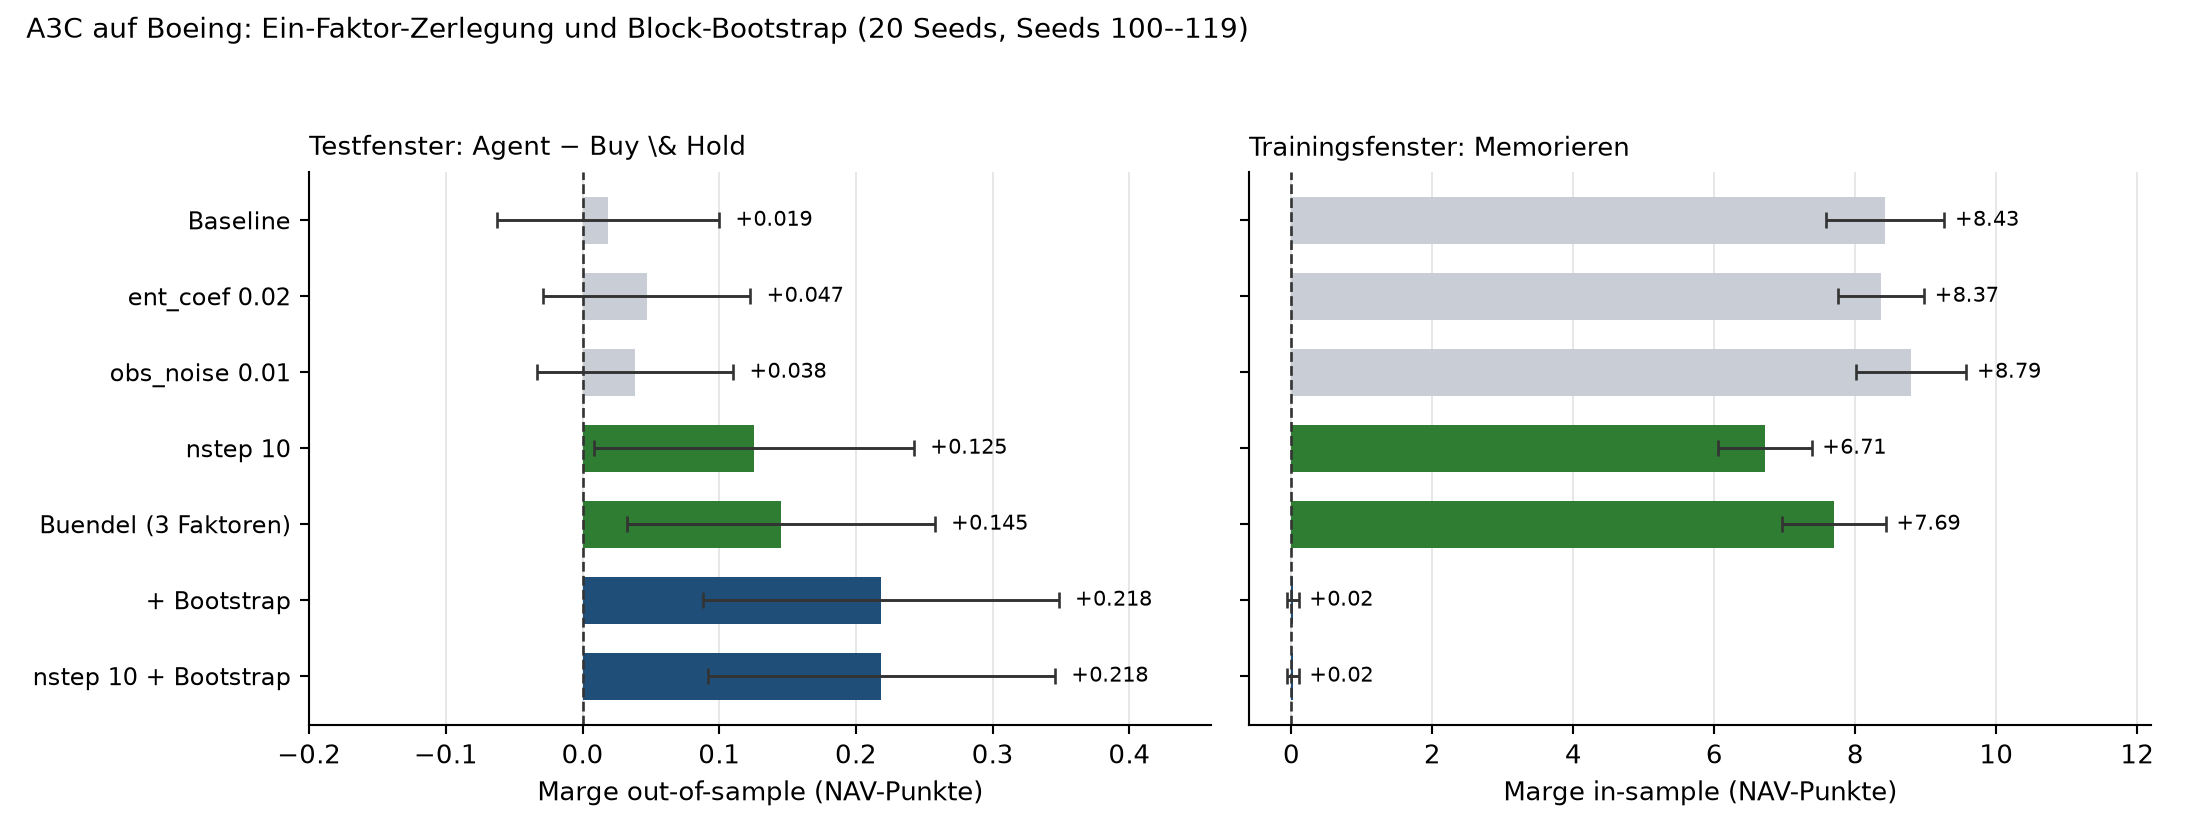
\includegraphics[width=\textwidth]{update_2026_a3c.png}
  \caption{Ein-Faktor-Zerlegung und Block-Bootstrap, 20 Seeds. Links die Testmarge
  (Fehlerbalken: 95-\%-KI), rechts die Marge im Trainingsfenster. Die beiden
  Bootstrap-Arme (dunkel) haben in-sample praktisch null Vorsprung und out-of-sample den
  größten.}
  \label{fig:a3c}
\end{figure}

\subsection{Was das Overfitting-Bild zeigt}

Abbildung~\ref{fig:a3c} macht den Kern sichtbar. Die vier Arme, die auf dem echten
Fenster trainieren, tragen in-sample zwischen $+6{,}7$ und $+8{,}8$ NAV-Punkte --- und
davon bleibt out-of-sample fast nichts. Die beiden Bootstrap-Arme haben in-sample
$+0{,}02$, also \emph{null} Vorsprung, und liefern gleichzeitig die besten Testwerte. Sie
haben den historischen Pfad nie gesehen; dass sie im Trainingsfenster nicht gewinnen, ist
deshalb keine Schwäche, sondern der Mechanismus. Ein In-Sample-Vorsprung von $+8$ ist
damit als das entlarvt, was er ist: Memorieren.

\subsection{Einschränkungen}

\paragraph{20 Seeds sind eine kleine Stichprobe.} Die Konfidenzintervalle in
Tabelle~\ref{tab:a3c-arms} sind breit, und der zentrale Bootstrap-Zuwachs ist mit
$p=0{,}26$ unterpowert. Belastbar ist: dass die Baseline keinen Vorsprung hat, dass
\texttt{nstep} $10$ das Bündel erklärt, dass die zwei übrigen Faktoren nichts tun, und
dass \texttt{nstep} $10$ $+$ Bootstrap die Baseline signifikant schlägt. Nicht belastbar
ist die Behauptung, der Bootstrap-Zusatz sei \emph{für sich} signifikant.

\paragraph{Nur fünf verschiedene synthetische Pfade.} Bei 20 Agenten und fünf
Bootstrap-Replikaten teilen sich je vier Seeds dieselbe synthetische Reihe. Die Seeds
variieren dann nur die Exploration, nicht die Umgebung. Ein Lauf mit einem eigenen Pfad
pro Agent wäre der nächste saubere Schritt.

\paragraph{Die In-Sample-Marge der Bootstrap-Arme ist nicht vergleichbar.} Sie wird auf
dem echten Fenster gemessen, auf dem diese Agenten nie trainiert haben; die Zeile ist
deshalb nur als Overfitting-Indikator lesbar, nicht als Leistungsmaß.

\paragraph{Daten und Umgebung.} Es gelten die Einschränkungen aus
Abschnitt~\ref{sec:abweichungen}: Beobachtungsvektor 334 statt 205, lokale CSVs statt
\texttt{yfinance}. A3C nutzt das gleiche Environment wie A2C, die Abweichungen wirken also
auf beide Arme gleichermaßen.

\subsection{Fazit des A3C-Teils}

Die Baseline bestätigt den A2C-Befund auf einem zweiten Algorithmus: kein belegbarer
Vorsprung vor Buy-and-Hold. Die Zerlegung zeigt, dass der Effekt der naheliegenden
``Regularisierung'' in Wahrheit aus der \textbf{Kredit-Zuweisung} stammt
(\texttt{nstep} $5\to10$); Entropie-Bonus und Beobachtungsrauschen sind in dieser
Größenordnung wirkungslos. Der \textbf{Block-Bootstrap} liefert als zweiter Hebel den
besten Testwert und den ersten signifikanten Vorsprung gegenüber der Baseline ---
allerdings erst in der Kombination. Konzeptionell ist das der interessantere Befund: Der
Agent braucht den realen historischen Pfad nicht, um auf dem Testfenster gleichauf oder
besser zu sein; viele plausible Pfade genügen.

\section{Artefakte und Reproduktion}

\begin{table}[H]
  \centering
  \caption{Artefakte des Updates.}
  \label{tab:artefakte}
  \small
  \begin{tabular}{ll}
    \toprule
    Datei & Inhalt\\
    \midrule
    \texttt{AIF\_Update\_2026.pdf} & dieser Report (aus LaTeX gebaut)\\
    \texttt{latex-update2026/} & LaTeX-Quelle des Reports (Tectonic)\\
    \texttt{UPDATE\_2026\_REPORT.md} & Markdown-Fassung desselben Inhalts\\
    \texttt{figs/update\_2026\_a2c.png}  & End-NAV je Episode, Training vs.\ Test (Boeing, 5 Seeds)\\
    \texttt{figs/update\_2026\_margins.png} & In-Sample- vs.\ Out-of-Sample-Marge je Aktie (20 Seeds)\\
    \texttt{figs/update\_2026\_a3c.png} & A3C: Ein-Faktor-Zerlegung und Block-Bootstrap (Boeing, 20 Seeds)\\
    \texttt{figs/update\_2026\_a3c\_replication.png} & A3C-Replikation: Out-of-Sample-Vorteil vs.\ Baseline, je Aktie + gepoolt\\
    \texttt{figs/update\_2026\_1y.png}   & Kursentwicklung der drei Aktien, letzte zwölf Monate\\
    \texttt{updated\_metrics\_final.json} & aktualisierte Fundamentalkennzahlen\\
    \texttt{results\_ba\_newdata.json}   & Roh-Ergebnisse Boeing (20 Seeds, Training + Test)\\
    \texttt{results\_air\_newdata.json}  & Roh-Ergebnisse Airbus (20 Seeds, Training + Test)\\
    \texttt{results\_tm\_newdata.json}   & Roh-Ergebnisse Toyota (20 Seeds, Training + Test)\\
    \texttt{results\_ba\_a3c*.json}   & A3C-Roh-Ergebnisse Boeing: Baseline, Ein-Faktor-Arme (\texttt{nstep10}, \texttt{ent02}, \texttt{noise01}), B\"undel, Bootstrap (20 Seeds)\\
    \texttt{results\_\{air,tm\}\_a3c*.json} & A3C-Roh-Ergebnisse Airbus/Toyota: Baseline, \texttt{nstep10}, \texttt{nstep10boot} (20 Seeds)\\
    \texttt{agent\_\{ba,air,tm\}\_1..20.zip} & die 60 neu trainierten A2C-Modelle\\
    \texttt{env\_runner.py}              & Environment-Aufsatz (lokale Daten, Seriell-Patch)\\
    \texttt{train\_eval\_multi.py}       & Training und Auswertung für beliebige Ticker, mit Resume\\
    \texttt{analyze\_seeds.py}           & Auswertung: Mittel, Streuung, 95-\%-KI, gepaarter $t$-Test\\
    \texttt{plot\_margins.py}            & Abbildung Train- vs.\ Testmarge je Aktie\\
    \texttt{train\_eval\_a3c.py}         & A3C-Training und -Auswertung (asynchron, n-Schritt-Returns, Block-Bootstrap)\\
    \texttt{plot\_a3c\_ablation.py}      & Abbildung A3C-Ein-Faktor-Zerlegung und Bootstrap\\
    \texttt{compare\_a3c\_repl.py}       & Replikations-Auswertung: gepaarte Tests je Aktie und gepoolt (AIR+TM)\\
    \texttt{plot\_a3c\_replication.py}   & Abbildung A3C-Replikation über die drei Aktien\\
    \texttt{train\_eval.py}              & Training und Auswertung (Notebook-Protokoll, 5 Agenten)\\
    \texttt{\{BA,AIR,TM\}\_5Y\_daily.csv} & Tagesdaten der drei Aktien (fünf Jahre)\\
    \bottomrule
  \end{tabular}
\end{table}

\paragraph{Reproduzieren.}
{\footnotesize
\begin{verbatim}
cd aif-latex
python3 aif_run/train_eval.py                  # Boeing, 5 Agenten, Notebook-Protokoll (~35 min)
python3 aif_run/train_eval_multi.py BA         # 20 Seeds, Boeing
sh aif_run/run_seeds20.sh                      # 20 Seeds fuer TM und BA
python3 aif_run/analyze_seeds.py TM BA AIR     # Tabellen + Signifikanztests
python3 aif_run/plot_margins.py                # Abbildung Train- vs. Testmarge
python3 aif_run/train_eval_a3c.py BA           # A3C auf Boeing, 20 Seeds (~2 h)
python3 aif_run/plot_a3c_ablation.py           # Abbildung A3C-Zerlegung + Bootstrap
python3 aif_run/compare_a3c_repl.py AIR TM     # Replikation: gepaarte Tests je Aktie + gepoolt
python3 aif_run/plot_a3c_replication.py        # Abbildung A3C-Replikation (3 Aktien)
cd paper/latex-update2026 && tectonic -X compile main.tex --outdir out   # Report-PDF
\end{verbatim}
}

Ein Lauf ist unterbrechbar: \texttt{train\_eval\_multi.py} überspringt Agenten, die bereits als
\texttt{.zip} vorliegen, und schreibt \texttt{results\_<ticker>\_newdata.json} inkrementell fort.

\paragraph{Hinweis zu den Datenquellen.} Yahoo/\texttt{yfinance} ist von diesem Host hart
geblockt (HTTP 429 auf allen Endpunkten, auch nach zwanzig Minuten). Boeing und Toyota
stammen daher aus der History-API von stockanalysis.com, die Airbus-Kurse aus der von Chris
nachgelieferten Yahoo-Reihe zu \texttt{AIR.PA} (Euronext Paris, in Euro). Achtung: der Endpunkt
\texttt{/api/symbol/s/AIR/history} liefert \emph{AAR Corp (US)} und nicht Airbus -- die
daraus zunächst abgeleiteten Airbus-Zahlen waren falsch und wurden verworfen.


\end{document}
